\newpage
\section{Appendix}

\subsection{Extended Related Work}\label{appendix:related}

A wave of recent work has applied Reinforcement Learning (RL) to improve the reasoning abilities of large language models (LLMs); often achieving state-of-the-art results on challenging tasks \citep{openai-o1, guo2025deepseek, seed2025seed1, carbonneaux2025cwm}. OpenAI's o1 series of models established that large-scale RL can substantially enhance long-horizon reasoning, but did not release any details on how these models were trained. Deepseek R1 (and R1-Zero) \citep{guo2025deepseek} provided the first comprehensive study on training high-performing and long Chain-of-Thought (CoT) models primarily via RL, documenting emergent behaviours under extended RL without any reliance on reward models \citep{lightman2023let} or Monte Carlo Tree Search (MCTS) \citep{xie2024monte}.

The earliest widely referenced RLVR (verifiable-reward) algorithm underlying this wave of reasoning development is Group Relative Policy Optimization (GRPO), introduced in \citet{shao2024deepseekmath}. GRPO is a critic-free, group-relative policy gradient with PPO-style clipping that replaces a learned value baseline with group baselines to reduce computational cost and stabilize credit assignment for long CoTs. While GRPO catalyzed rapid progress, subsequent work document its limitations (token-level clipping, model collapse risks) and motivate different group- or sequence- level variants \citep{yu2025dapo, yue2025vapo, hu2025open, gspo}.

\citet{yu2025dapo} propose the Decoupled clip and Dynamic Sampling Policy Optimization (DAPO), where they decouple $\eps_{\texttt{low}}$ and $\eps_{\texttt{high}}$ clipping in the GRPO objective and do \textit{Clip-Higher} for $\eps_{\texttt{high}}$ to avoid entropy collapse. Furthermore, they do dynamic sampling of prompts in a given batch to avoid samples with zero variance (or advantage) which contribute zero policy gradients. Finally, they employ token-level loss aggregation unlike GRPO, which uses sample-level loss averaging. With these modifications, they are able to surpass the vanilla GRPO baseline while avoiding entropy collapse in the RL training. In parallel, \citet{yue2025vapo} develop VAPO; a value-augmented PPO tailored for long CoTs with strong stability and outperforming value-free baselines like GRPO and DAPO. They combine value pre-training and decoupled Generalized Advantage Estimation (GAE) from VC-PPO \citep{yuan2025s}, loss objective modifications from DAPO, and propose length-adaptive GAE to come up with an open recipe, VAPO, that has been used to train large MoE models in \citet{seed2025seed1}. Similarly, other technical report like Magistral \citep{rastogi2025magistral}, Kimi-k1.5 \citep{team2025kimi}, Minimax-01 \citep{li2025minimax} detail various details on their RL training recipes, but don't share extensive experiments on why their design choices are better than the baselines.

\subsection{RL for LLMs: GRPO and DAPO}\label{appendix:background}

\paragraph{Group Relative Policy Optimization~(GRPO)}
GRPO~\citep{shao2024deepseekmath} adapts PPO~\cite{schulman2017ppo} for LLM fine-tuning with verifiable rewards. 
For a given prompt $x$, the old policy $\pi_{\text{gen}}(\theta_{\text{old}})$ generates $G$ candidate completions $\{y_i\}_{i=1}^G$, each assigned a scalar reward $r_i$. 
To emphasize relative quality within the group, rewards are normalized as
\begin{equation}
    \hat{A}_i = \frac{r_i - \mathrm{mean}(\{r_j\}_{j=1}^G)}{\mathrm{std}(\{r_j\}_{j=1}^G) + \epsilon}. \label{eq:advantage}
\end{equation}
Each completion $y_i$ of length $|y_i|$ contributes at the token level through ratios
\begin{equation}
    \rho_{i,t}(\theta) = \frac{\pi_{train}(y_{i,t} \mid x, y_{i,<t},\theta)}{\pi_{gen}(y_{i,t} \mid x, y_{i,<t}, \theta_{\text{old}})}
\end{equation}
The GRPO objective averages across both completions and tokens:
\begin{equation}
    \mathcal{J}_{\mathrm{GRPO}}(\theta) 
    % = \mathbb{E}_{x \sim D,\, \{y_i\}_{i=1}^G \sim \pi_{gen}(\cdot \mid x, \theta_{\text{old}})} 
    = \mathbb{E}_{\begin{subarray}{l} \, x \sim D, \\ \{y_i\}_{i=1}^G \sim \pi_{\text{gen}(\cdot \mid x, \theta_{\text{old}})} \end{subarray}}
    \left[ \frac{1}{G} \sum_{i=1}^G \frac{1}{|y_i|} \sum_{t=1}^{|y_i|}
    \min\!\left( \rho_{i,t}(\theta)\hat{A}_i,\; \mathrm{clip}(\rho_{i,t}(\theta), 1\pm \epsilon)\hat{A}_i \right) \right]
\end{equation}
Thus GRPO preserves token-level policy ratios as in PPO, while using sequence-level, group-normalized advantages to stabilize learning under sparse rewards.

\paragraph{Decoupled Clip and Dynamic Sampling Policy Optimization (DAPO)}
DAPO~\citep{yu2025dapo} extends GRPO with two key modifications.  
First, it replaces symmetric clipping with \emph{asymmetric clipping}, using distinct thresholds for upward and downward deviations: $\mathrm{clip}_{\mathrm{asym}}(\rho, a) = \mathrm{clip}(\rho,\, 1-\epsilon^-, 1+\epsilon^+) $, where $\epsilon^-$ and $\epsilon^+$ are hyper-parameters.

Second, DAPO changes the aggregation scheme to operate at the \emph{prompt level}.  
For a given prompt $x \sim D$, the old policy produces $G$ completions $\{y_i\}_{i=1}^G$ with advantages $\{\hat{A}_i\}$ (\Cref{eq:advantage}).  
Let $T = \sum_{i=1}^G |y_i|$ denote the total number of tokens across all completions.  
With token-level ratios as in \Cref{eq:is}.
The DAPO surrogate objective is
\begin{equation}
\mathcal{J}_{\mathrm{DAPO}}(\theta) 
% = \mathbb{E}_{\substack{x \sim D, \\ \{y_i\}_{i=1}^G \sim \pi_{gen}(\cdot \mid x, \theta_{\text{old}})}} 
= \mathbb{E}_{\begin{subarray}{l} \, x \sim D, \\ \{y_i\}_{i=1}^G \sim \pi_{\text{gen}(\cdot \mid x, \theta_{\text{old}})} \end{subarray}}
\left[ \frac{1}{T} \sum_{i=1}^G \sum_{t=1}^{|y_i|}
\min\!\left( \rho_{i,t}(\theta)\hat{A}_i,\; \mathrm{clip}_{\mathrm{asym}}(\rho_{i,t}(\theta))\hat{A}_i \right) \right]. \label{eq:dapo_loss}
\end{equation}
This prompt-level normalization ensures that each token contributes equally to the prompt's loss, regardless of the number or length of its sampled completions.
DAPO also introduces dynamically dropping 0-variance prompts from the batch during training and filling the batch with more prompts until the batch is full. We skip that change here since its effect is similar to having a larger batch size.


\subsection{Training Setup}\label{appendix:setup}

\paragraph{Datasets}
For small-scale SFT, we use a curated data mix of reasoning traces. 
We filter this dataset by removing trivial prompts, discarding solution traces exceeding $12k$ tokens, and decontaminating with AIME 2024/2025 \citep{aime} and MATH-500 \citep{hendrycks2021measuring} benchmarks. For the RL stage, we use the Polaris-53K dataset~\citep{polaris2025} for most of our runs; additionally using the Deepcoder dataset \citep{deepcoder2025} for runs with both math and code.

\paragraph{Supervised Fine-tuning}
We run SFT using a batch size of 2M tokens, max sequence length of 12288, and a learning rate of $3 \times 10^{-5}$ using the AdamW optimizer \citep{adamw} on 32 H100 GPU nodes for approximately 4 epochs and 32B tokens in total.

\paragraph{Reinforcement Learning}
We allocate $14$k generation budget during RL training, where $12\text{k}$ tokens are allocated to the intermediate reasoning (``thinking''), followed by $2\text{k}$ tokens for the final solution and answer. We sample $48$ prompts in each batch, each with $16$ generations per prompt. Thus, we get the total batch size as $768$ completions per gradient update step. The rewards are given as $\pm 1$ to correct and incorrect traces respectively. We use a constant learning rate of $5 \times 10^{-7}$, AdamW optimizer \citep{adamw} with $\epsilon = 10^{-15}$, weight decay of 0.01 (default in AdamW), and a linear warmup of 100 steps. The lower $\epsilon$ is to avoid gradient clipping (epsilon underflow)~\citep{wortsman2023stable}.

We use automated checkers like Sympy \citep{meurer2017sympy} or Math-Verify\footnote{https://github.com/huggingface/Math-Verify} for assessing the correctness of the final answer for math problems after stripping out the thinking trace ($\texttt{<think>}\cdots\texttt{</think>}$). We use a custom code execution environment for coding problems involving unit tests and desired outputs.

We used 80 Nvidia GB200 GPU for a single run, with a compute budget ranging from 3.5-4K GPU hours for establishing different design choices in \Cref{sec:fwd_ablations}, 16K for the leave-one-out experiments (\Cref{sec:loo}), and finally 30k-100K GPU hours for our larger scale runs (\Cref{sec:diff_axes}). We adopt a generator–trainer split between GPUs. For 80 GPU experiments, we set $64$ of those as \emph{generators}, responsible for the generation of reasoning trace using the optimized inference codebase. The remaining 16 GPUs act as \emph{trainers}, which receive generated trajectories, perform policy updates, and periodically broadcast updated parameters back to the generators.

\subsection{What curve to fit?} \label{appendix:curve_to_fit}
Pre-training curves are usually fit using power-law equation~\citep{misfitting,kaplan2020scaling,scalingdataconstrained}, which in our case would model performance as $R_{C} = A - D/C^B, C\geq C_0$, where $D$ is a constant, and $C_0$ marks the compute threshold beyond which the law holds.
Intuitively, this implies that each multiplicative increase in compute yields a constant proportional gain in performance.
For RL post-training, however, we find a sigmoidal fit (\cref{eq:sigmoid_law}) more appropriate for several reasons.
First, for bounded metrics such as accuracy or reward, sigmoidal curves provide better predictive fits~\citep{ruan2024,srivastava2022bigbench}; we observe the same, with accurate extrapolation to higher compute (\Cref{fig_100k_main}).
Second, power laws are unbounded at low compute and are typically fit only beyond a threshold $C_0$. In RL, where total training spans far fewer steps (e.g., only $\sim$75 evaluation points to fit only in \Cref{fig_100k_main}), discarding early points a lot further reduces the already limited data available for fitting.
Third, empirically, sigmoidal fits are substantially more robust and stable than power-law fits.
Concretely, consider the $100\text{k}$ GPU-hour run on the 8B dense model shown in \Cref{fig_100k_main}.
When we fit a power-law curve between $1.5\text{k}$–$50\text{k}$ GPU hours, it predicts an asymptotic performance of $A = 1.0$, which is clearly incorrect - the actual curve saturates near $0.65$.
In contrast, the sigmoidal fit yields an accurate prediction of $A = 0.645$.
Moreover, the power-law fit is highly sensitive to the chosen fitting regime: fitting over $(5\text{k}, 50\text{k})$ GPU hours instead gives $A = 0.74$, while the sigmoidal fit remains robust and still predicts $A = 0.645$.
Power-law models only recover the correct asymptote when fitted exclusively in the high-compute regime (e.g., $30\text{k}$–$60\text{k}$ GPU hours).
However, our goal is to predict large-scale performance from lower-compute regimes, where such long runs are unavailable.


Given these considerations, we use the sigmoidal form throughout our analysis. Intuitively, a sigmoidal curve captures saturating returns - grows slowly in the low-compute regime, accelerates sharply through a mid-range of efficient scaling, and then saturates at high compute as it approaches a finite performance ceiling.

One thing to note is that at high compute regime, sigmoidal curve behaves same as power-law. Concretely, we can have the following approximation of sigmoidal curve:
\begin{align*}
    R_C &= R_0 + \frac{A-R_0}{1 + (C_{mid}/C)^B} && \text{(sigmoidal curve from \cref{eq:sigmoid_law})} \\
    \implies R_C &\approx R_0 + (A-R_0)\left(1-\frac{C_{mid}^B}{C^B}\right) && \text{(For $C >> C_{mid}$, high compute regime)}\\
    &= A - \frac{(A-R_0)C_{mid}^B}{C^B}\\
    &= A - \frac{D}{C^B}
\end{align*}
where above $D = (A-R_0)C_{mid}^B$. And this is the same form of power-law mentioned at the start of this section.

\subsection{Fitting scaling curves} \label{appendix:fitting_curves}
We fit the sigmoid-law equation in \Cref{eq:sigmoid_law} to the mean reward on our held-out validation set. 
This set consists of $1,000$ prompts held out from the Polaris-53k~\citep{polaris2025} math dataset, with $16$ generations sampled every evaluation step performed at $100$ steps intervals. 

Directly fitting all three parameters $\{A,B,C_{mid}\}$ is challenging. 
Instead, we perform a grid search over $A \in \{0.450, 0.455, 0.460, \ldots, 0.800\}$ and $C_{mid}\in [100, 40000]$ (searching over 100 linearly separated values), and for each candidate $A, C_{mid}$ fit $B$. 
The best fit (measured by sum of squared residuals) across this grid is selected as the final curve. 
We use SciPy’s \texttt{curve\_fit} with default initialization; varying the initialization strategies produced identical results. To enable future studies to fit compute–performance RL scaling curves, we release a minimal code repository at \href{https://www.devvrit.com/scalerl_curve_fitting}{www.devvrit.com/scalerl\_curve\_fitting}.

To estimate the error margin of our fits, we trained three independent \scalerl\ runs with a batch size of $768$ and generation length of $14\text{k}$ (as used in \Cref{sec:loo}), shown in \Cref{fig:error_margin}. 
We found that the fit values of $A$ varied by at most $\pm 0.015$, suggesting $0.02$ as a reasonable error margin on the estimates of asymptotic performance. Estimating the error margin for the fitted value $B$ is difficult, as different algorithms with different $A$ values can have different error margins for $B$. However, for the purpose of comparing algorithms, we can safely deduce that if two methods achieve similar $A$ values (within $0.02$), the one with higher $B$ when a refit is done with the average of $A$ values is at least as good in terms of efficient scalability.

\subsection{Comparing algorithms} \label{appendix:comparing_algos}
Consistent with observations in large-scale pre-training, where the loss exhibits a sharp initial drop before settling into a predictable power-law decay~\citep{misfitting}, we observe a similar two-phase behavior in RL. The mean reward increases rapidly, almost linearly, during the $\sim$first epoch ($\sim 1\text{k}$ steps, or $\sim$1.5k GPU Hours for most runs), after which the curve follows sigmoidal-law behavior (see \Cref{fig:appendix_loo} to see the ``sigmoid" like curve). Our sigmoidal-law fits are applied to this latter portion of the training curve. 

Unlike pre-training, our main goal is not to predict the performance of a fixed recipe, but to identify which algorithms and design choices scale reliably, and to design algorithm that exhibits predictive nature. Achieving highly robust fits typically requires very large runs with hundreds or thousands of evaluation points, which is impractical in our setting for two reasons. First, running all ablations at such scale would be computationally prohibitive. Second, many RL algorithms we compare are themselves not scalable to such extreme budgets: they often saturate much earlier or even degrade with more compute due to instability. For example, our baseline method (\Cref{sec:fwd_ablations}) destabilizes beyond $\sim 3500$ GPU-hours, since overlong generation truncations exceed $10\%$ of generations - reducing the effective batch size. More discussion on this is in \Cref{appendix:truncations}. 

As we ablate across different axes in \Cref{sec:fwd_ablations}, we discover design choices that improve stability at higher compute. Some ablated variants can scale further, e.g., $\sim 5\text{k}$ GPU hours for $\epsilon=0.26$ in DAPO, $\sim 6\text{k}$ GPU hours with the FP32 precision fix (\Cref{sec:fp32}), and $\sim 7\text{k}$ GPU hours for CISPO. Once we combine the best design choices, we obtain a stable and scalable recipe, which allows us to run leave-one-out (LOO) experiments for $\sim 1600$ GPU hours per run.

\subsection{Robustness of fits} \label{appendix:fits_robustness}
One may wonder how robust our fitted curves are. We address a few relevant points below:

\begin{itemize}
    \item For stable and scalable experiments, including all runs from \Cref{sec:loo} onward, changing the fitting regime (e.g., including or excluding the initial $1.5$k GPU-hour range) yields similar predictable results.
    For instance, in the 100k GPU-hour run on the 8B dense model, fitting over $(1.5\text{k}, 50\text{k})$ gives $B = 1.70$, $A = 0.645$, while $(0, 100\text{k})$ gives $B = 1.56$, $A = 0.655$, $(0, 50\text{k})$ gets $B=1.7, A=0.645$, and $(5\text{k}, 50\text{k})$ gives $B = 1.67$, $A = 0.645$. Across these regimes, parameter values remain within the expected error margin (\Cref{sec:conclusion}).

    \item We nonetheless skip the low-compute regime because early training phases, especially in less stable setups from \Cref{sec:fwd_ablations}, often plateau prematurely or deviate from the sigmoidal trend due to transient instabilities (see Appendix~\ref{appendix:comparing_algos}, \ref{appendix:truncations}).
    Excluding this region allows the fit to focus on the mid-to-high compute range where saturation behavior is clearer and more consistent.

    \item The $1.5$k GPU-hour threshold is a heuristic chosen empirically: it approximately corresponds to one epoch for most experiments in \Cref{sec:fwd_ablations}.
    Larger cutoffs reduced the number of fitting points, while smaller ones often introduced noise.
    We found $1.5$k GPU hours to provide the best balance between fit stability and sample coverage, consistent with practices of skipping low-FLOPs regime in pre-training scaling analyses and fitting~\citep{misfitting}.

\end{itemize}

% \subsection{Robustness of fits}
% One may wonder how robust our fits are. We address a few relevant points here:
% \begin{itemize}
%     \item For most of the experiments that are stable and scale well, including all the runs in \Cref{sec:loo} and onward, changing the fitting regime to start from 0 (i.e., without skipping the initial 1.5k GPU hours) produces as stable and predictable fits as done currently after skipping the initial small 1.5 GPU hour regime. Concretely, taking example of the 100k GPU-hour run on 8B Dense model - fitting on (1.5k, 50k) regime gives fitted values of $B=1.7, A=0.645$. 
%     Changing this to (0, 100k) gives $B=1.56, A=0.655$. For (0, 50k) we get $B=1.7, A=0.645$. Changing this to (5k, 50k) gives $B=1.67, A=0.645$. So we see that for different fitting regimes, we get similar values within error margin (\Cref{sec:conclusion}).
%     \item The reason we still choose to skip low-compute regime is because some of the initial runs in \Cref{sec:fwd_ablations}, which were not as stable and scalable (talked about more in Appendix~\ref{appendix:comparing_algos} and Appendix~\ref{appendix:truncations}), plateaued abruptly and early, not fully following the sigmoidal fits throughout. Skipping the initial low-compute regime helped us focus on the latter part of mid to high compute range and get better fits following the saturation at higher compute. 
%     \item The choice of skipping the initial low-compute regime being $1.5$k GPU hours is somewhat heuristics. The choice was based on skipping the 1st epoch, which was approximately $1.5$k GPU hours for most of the experiments in \Cref{sec:fwd_ablations}. Changing this to much more than 1.5k GPU hours led to less points available to fit onto, and changing it to less than 1.5k GPU hours sometimes led to noisy fits. We found the 1.5k GPU Hour to be the best balanced in terms of total number of points available to fit onto while also not considering the initial low-compute regime, as is also done in pre-training~\citep{misfitting}.
% \end{itemize}





\subsection{Interpreting Sigmoidal Curves} \label{appendix:interpreting_fit}


\begin{figure*}[h]
    \centering
    \subfloat[]{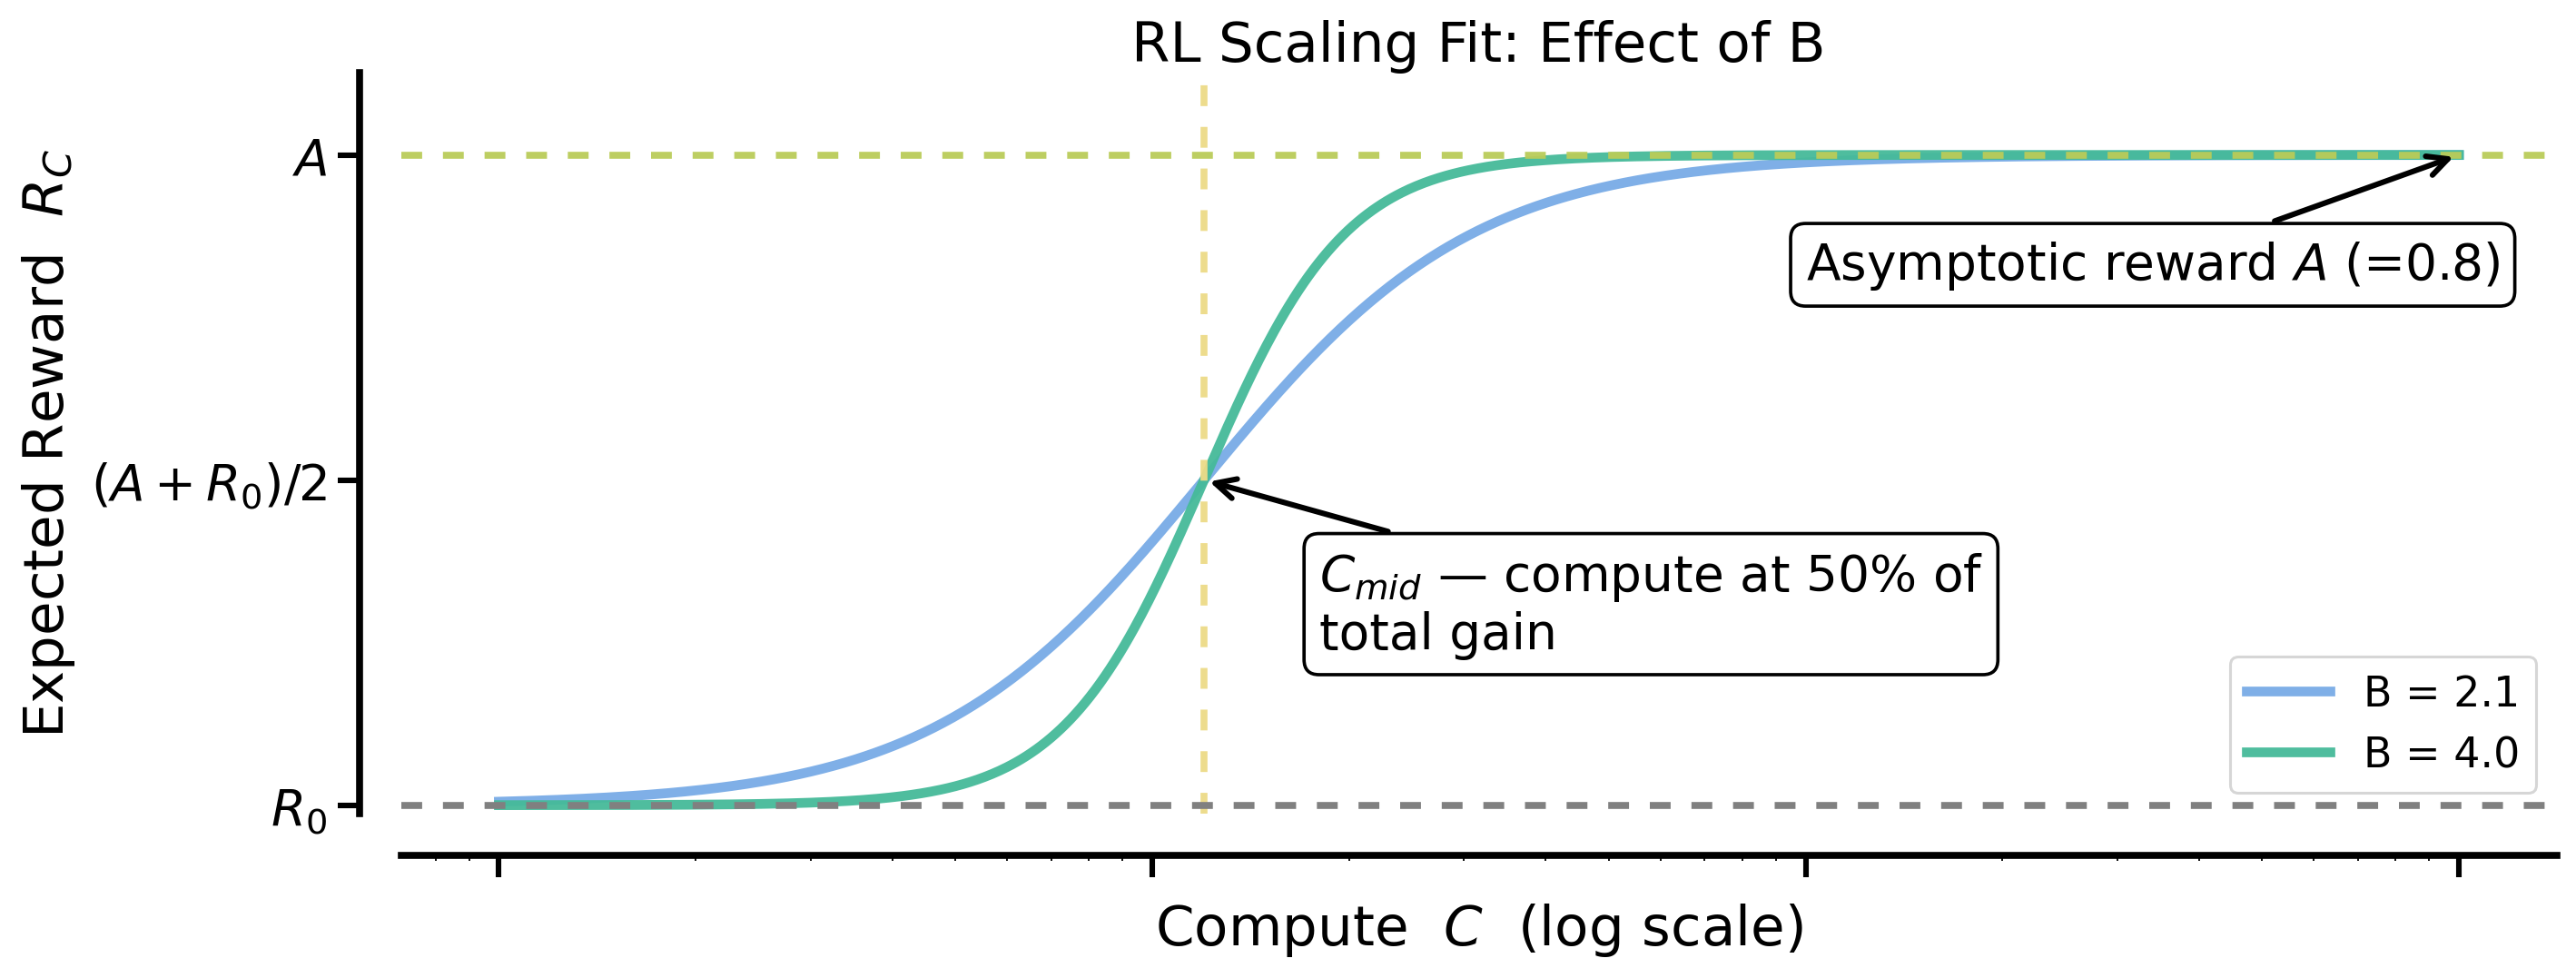
\includegraphics[width=0.48\textwidth]{paper_figs/effect_of_B.png} \label{fig:effect_of_B}}
    \hfill
    \subfloat[]{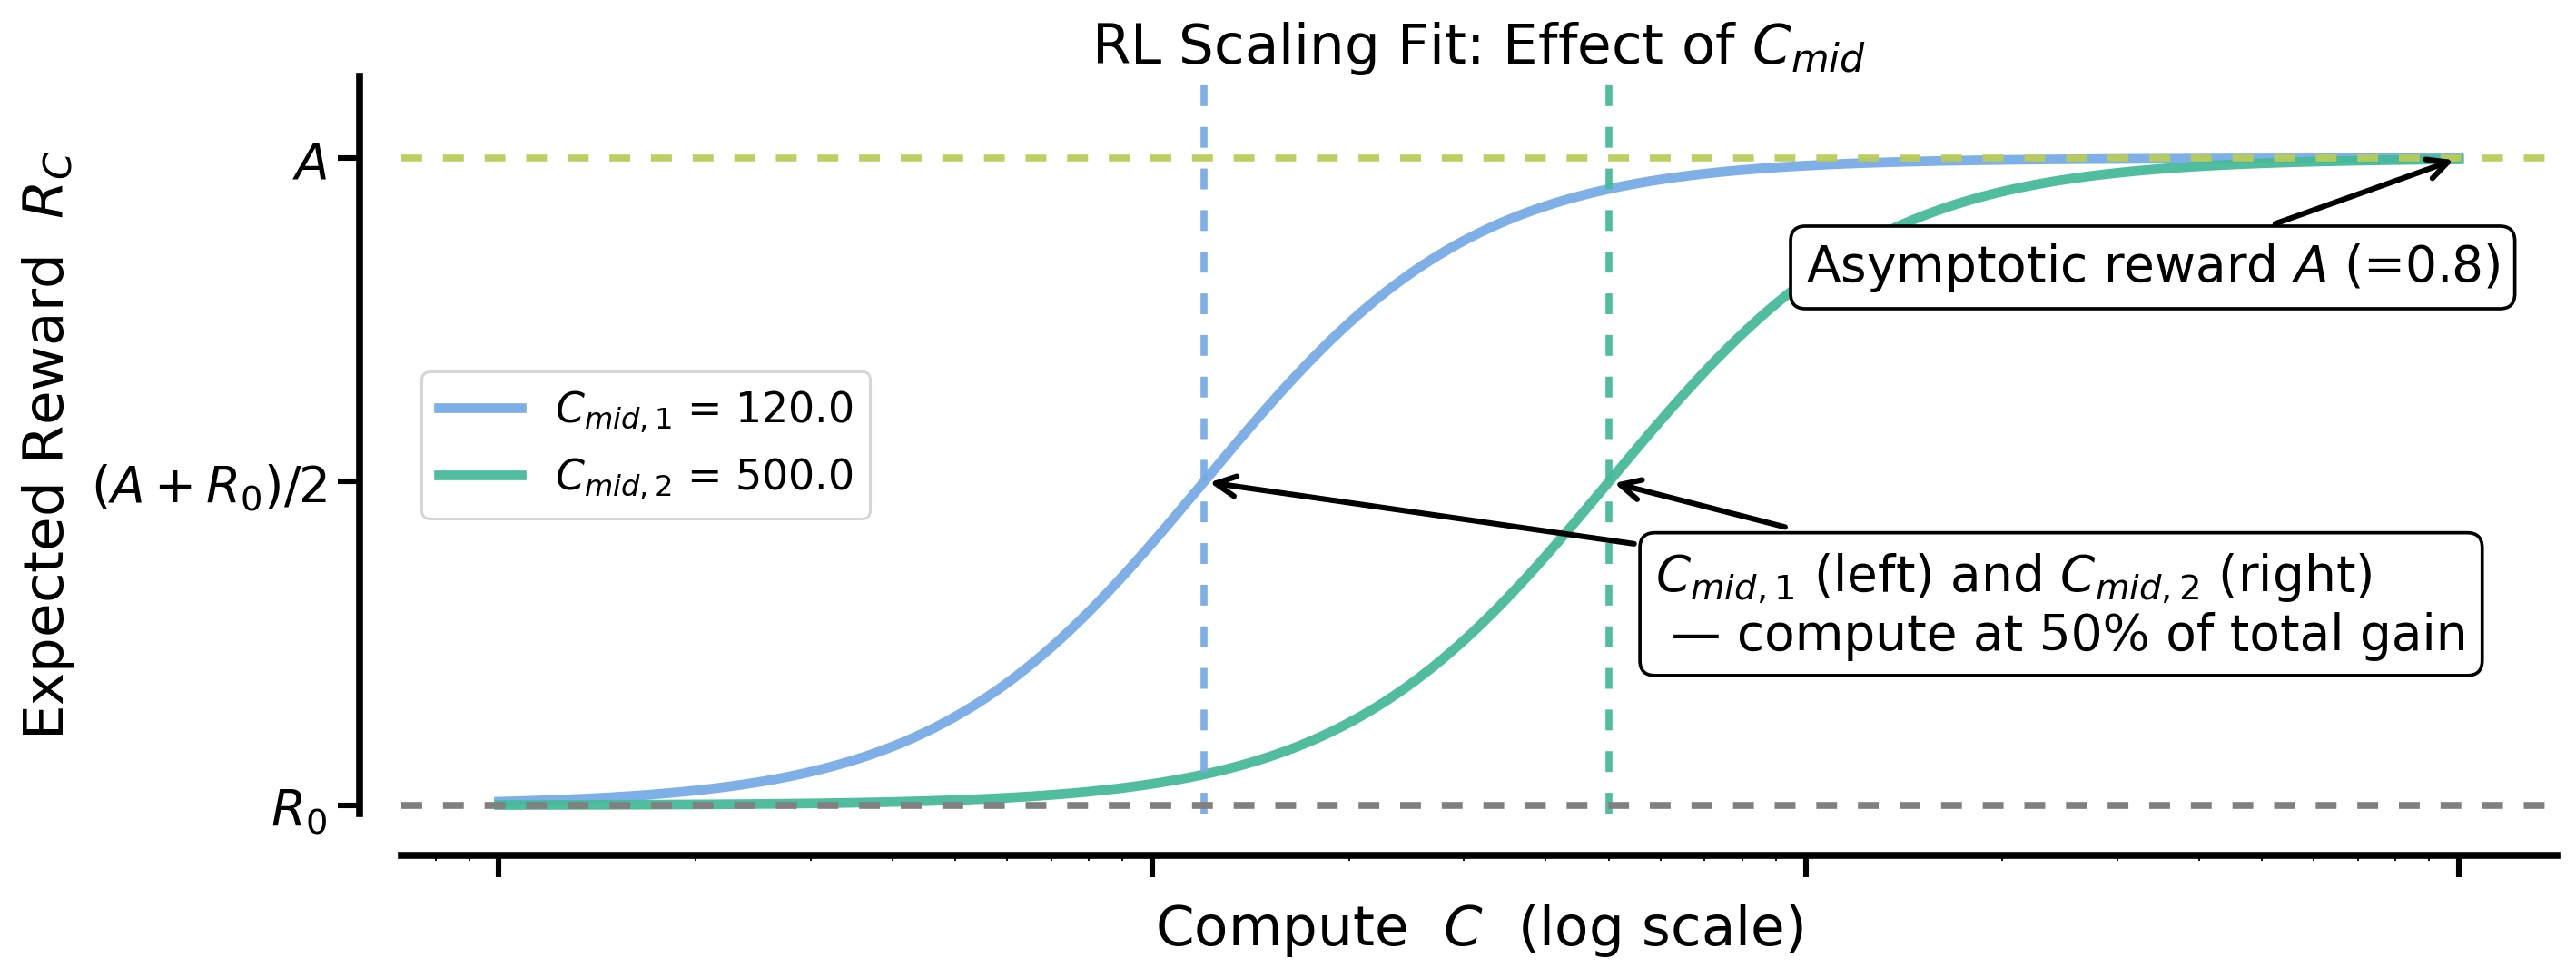
\includegraphics[width=0.48\textwidth]{paper_figs/effect_of_Cmid.png} \label{fig:effect_of_Cmid}} 
    \hfill
    \caption{\small Keeping all parameters same and only changing (a) $B$, (b) $C_{mid}$. Both these parameters modulate the efficiency of the training run.}
\end{figure*}

\begin{figure*}[h]
    \centering
    \subfloat[]{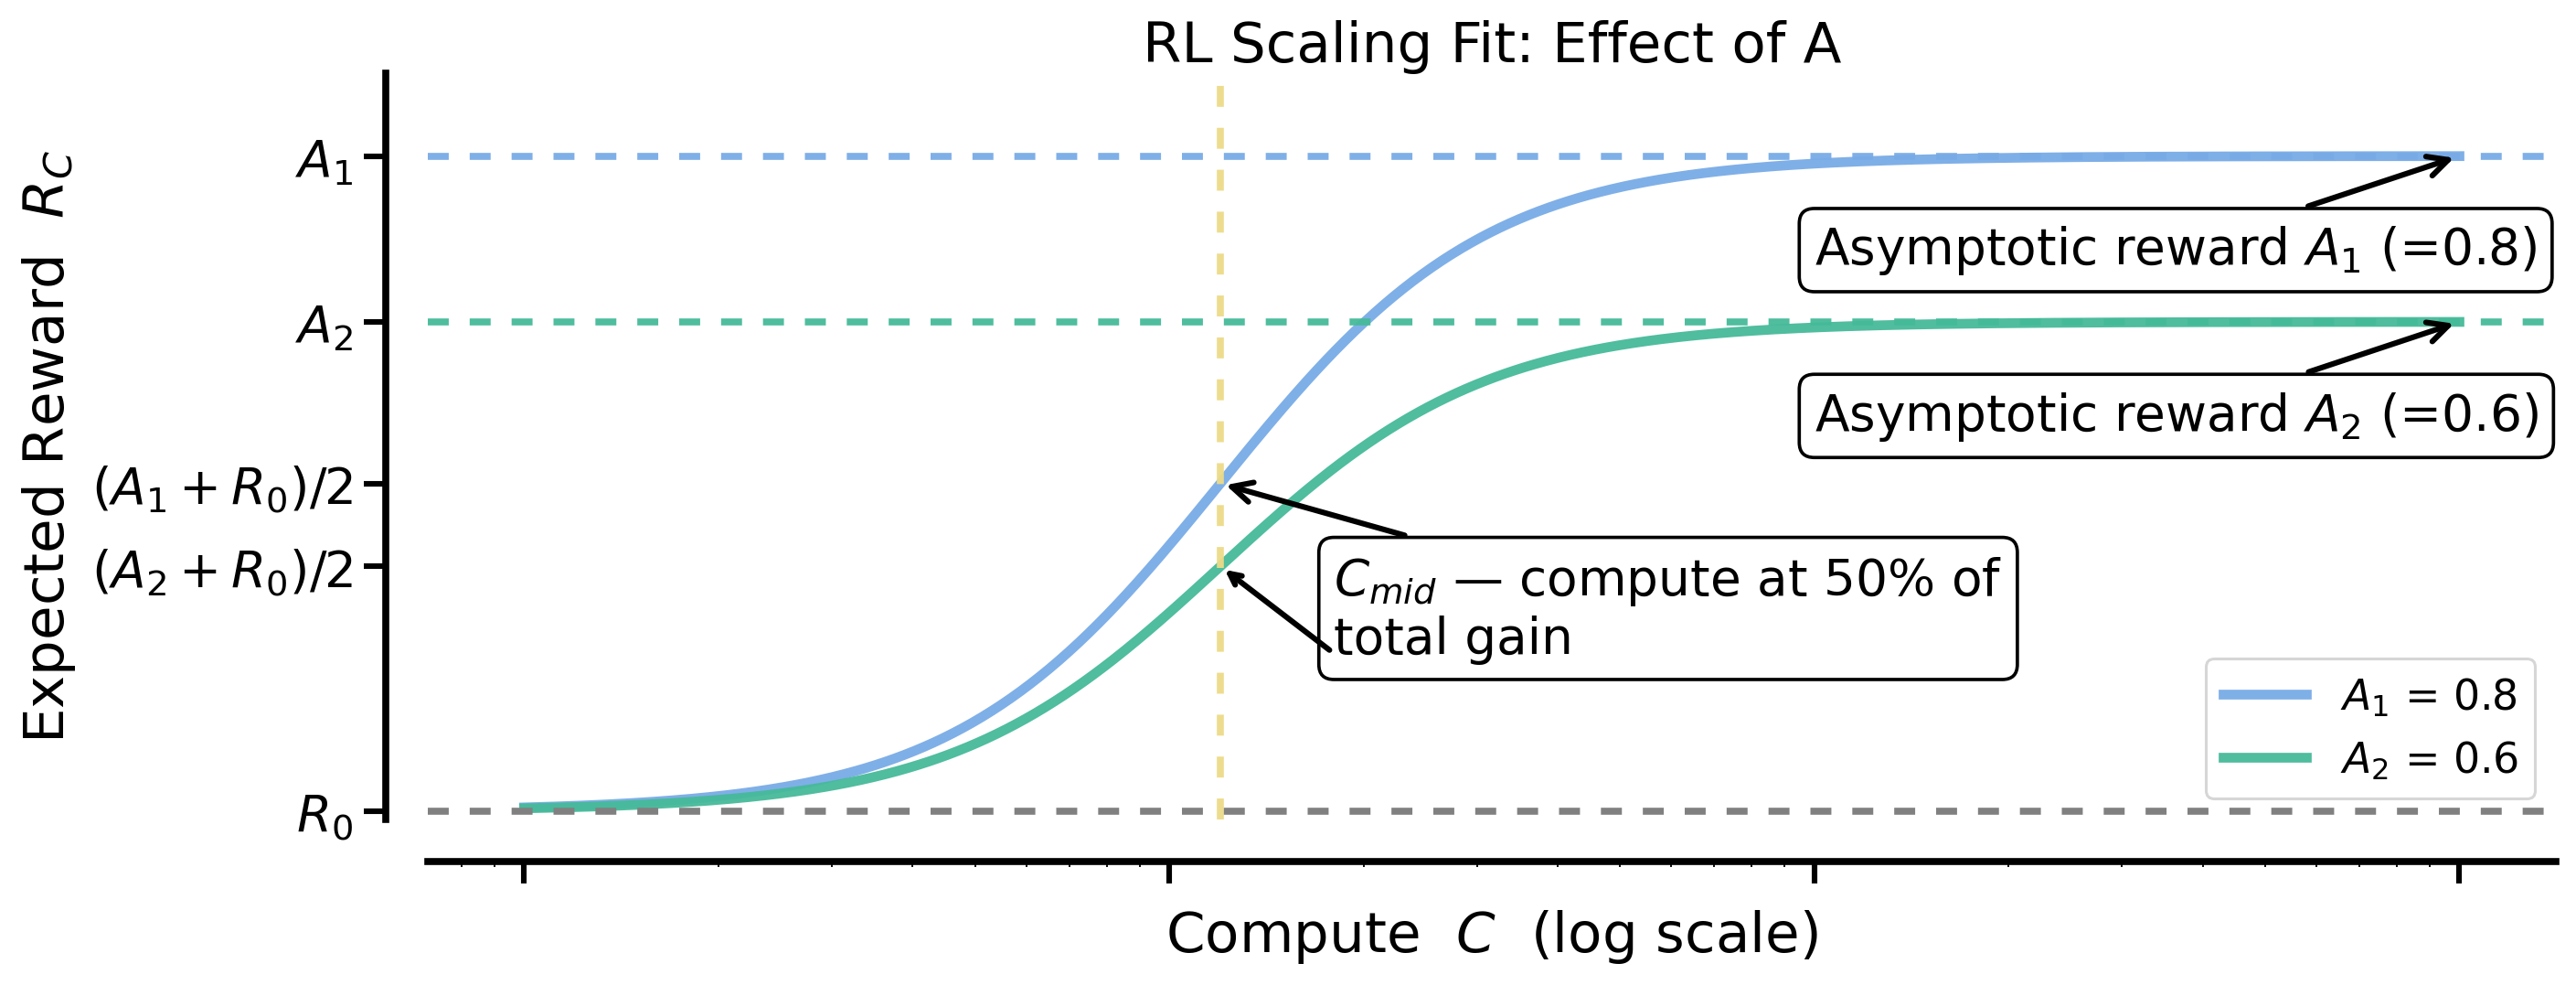
\includegraphics[width=0.48\textwidth]{paper_figs/effect_of_A.png} \label{fig:effect_of_A}}
    \hfill
    \subfloat[]{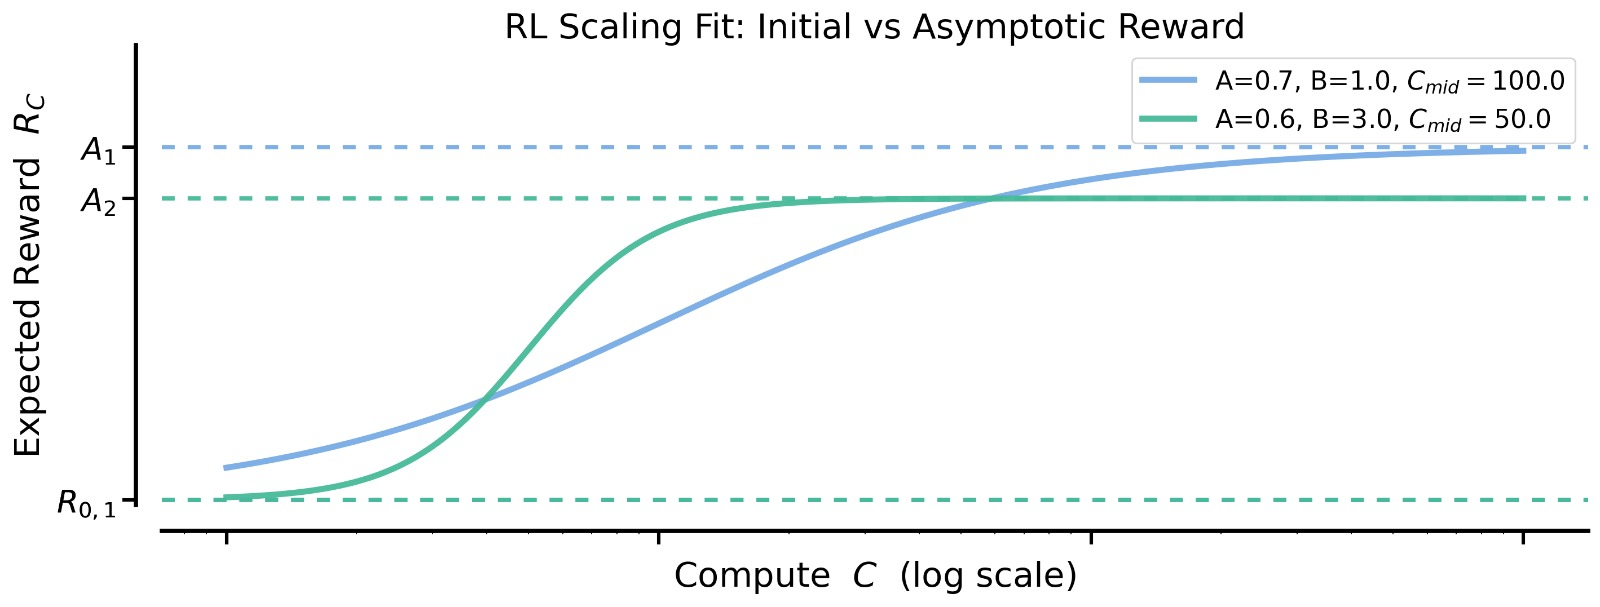
\includegraphics[width=0.48\textwidth]{paper_figs/slow_horse.jpeg} \label{fig:slow_horse}} 
    \hfill
    \caption{\small (a) Keeping all parameters same and only changing $A$.  
    (b) A design choice can be less efficient yet reach a higher asymptote. When designing scalable methods, one should prioritize choices that raise the asymptotic ceiling $A$, since the ultimate goal is maximizing performance at scale.}
\end{figure*}

\Cref{fig:interpreting_fit} presented an example fit illustrating the influence of parameters $A$, $B$, and $C_{\text{mid}}$.
Here, we extend this with additional illustrations: \Cref{fig:effect_of_B}, \Cref{fig:effect_of_Cmid}, and \Cref{fig:effect_of_A} vary $B$, $C_{\text{mid}}$, and $A$ respectively, while keeping the other parameters fixed.
We observe that $B$ and $C_{\text{mid}}$ primarily affect the \emph{efficiency} of scaling, whereas $A$ determines the asymptotic performance achievable at large compute.
In \Cref{fig:slow_horse} we see a case of two runs where one is much more efficient, hence shows initial promising gains, but converges to a lower asymptote, while the other progresses more slowly yet ultimately surpasses it due to a higher $A$.
In practice, scaling strategies should prioritize design choices that raise the asymptotic ceiling $A$, and only then optimize for efficiency parameters such as $B$ or $C_{\text{mid}}$.

\subsection{Forward and LOO Ablations}\label{appendix:forward}
We show additional results for \Cref{sec:fwd_ablations} in Figures \ref{fig:loss_agg}-\ref{fig:adv_norm}.
We also plot the pass rate vs compute leave one out experiments from \Cref{sec:loo}  in \Cref{fig:appendix_loo}.

\begin{figure*}[h]
    \centering
    \subfloat[]{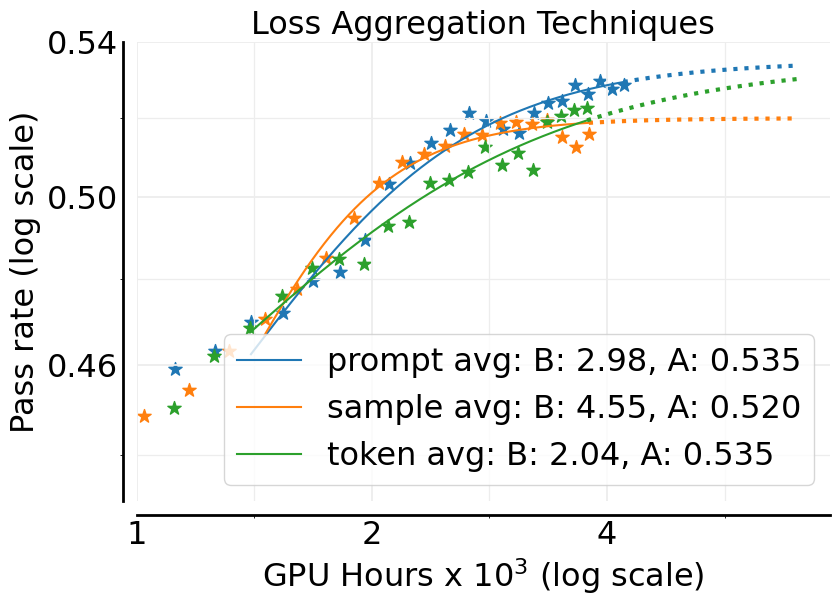
\includegraphics[width=0.45\textwidth]{paper_figs/loss_agg.png} \label{fig:loss_agg}}
    \hfill
    \subfloat[]{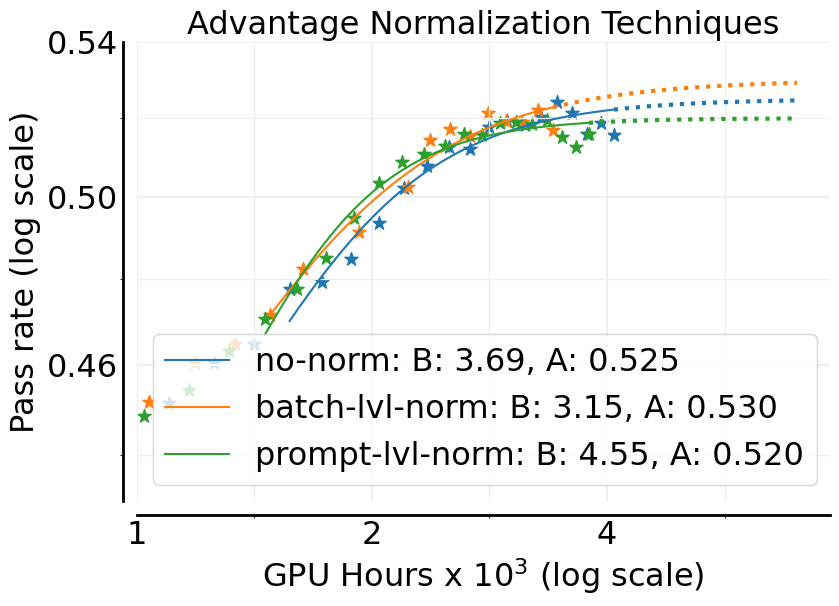
\includegraphics[width=0.45\textwidth]{paper_figs/adv_norm.png} \label{fig:adv_norm}} 
    \hfill
    \caption{\small Comparing (a) loss aggregation, (b) different advantage normalization techniques.}
\end{figure*}

 

\begin{figure*}[h]
    \centering
    \subfloat[]{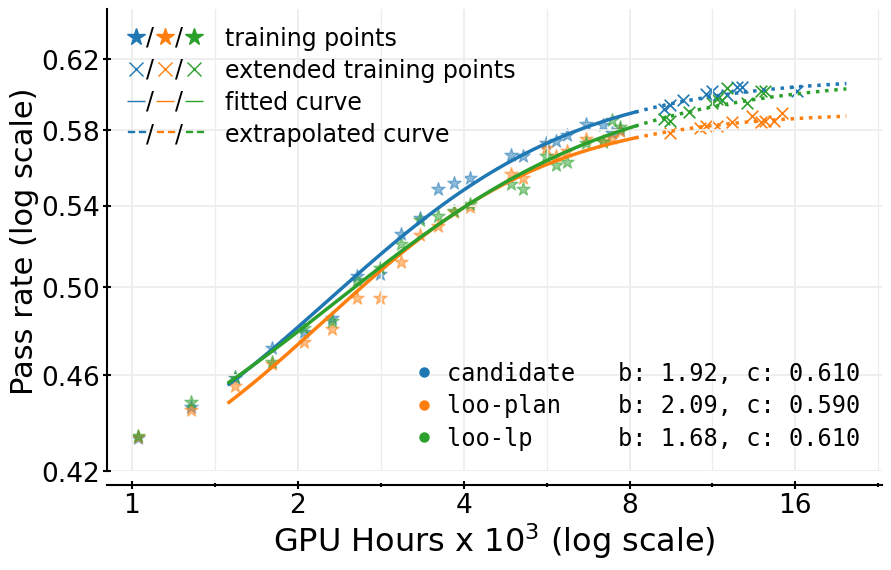
\includegraphics[width=0.32\textwidth]{paper_figs/loo_1.png} \label{fig:loo_1}}
    \hfill
    \subfloat[]{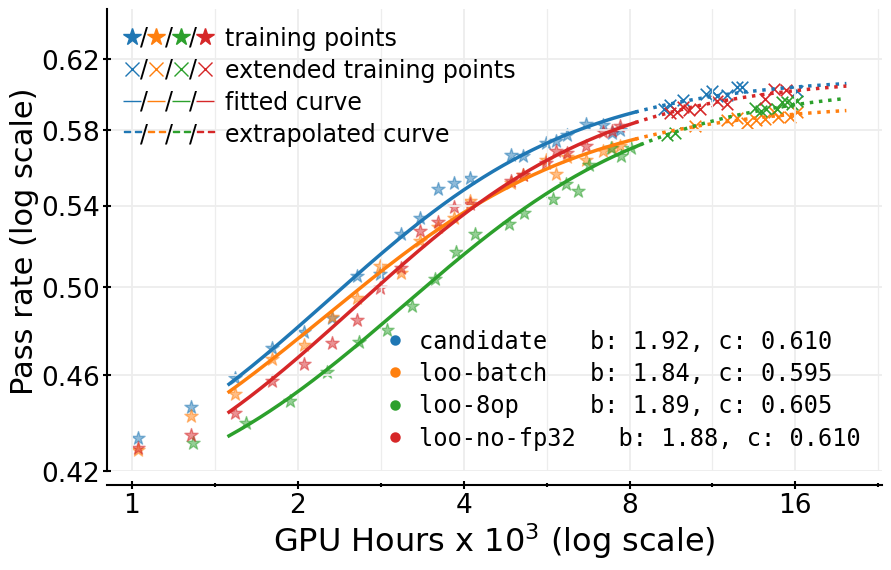
\includegraphics[width=0.32\textwidth]{paper_figs/loo_2.png} \label{fig:loo_2}} 
    \hfill
    \subfloat[]{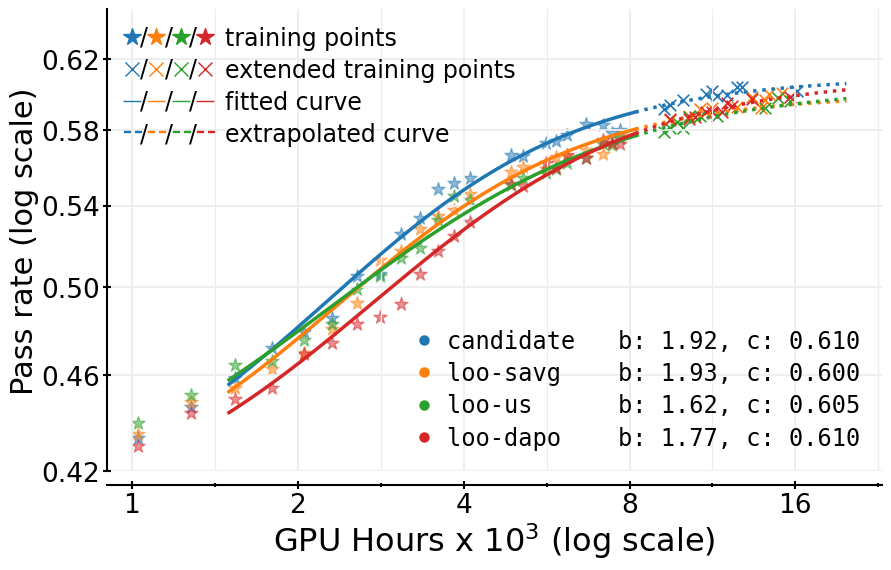
\includegraphics[width=0.32\textwidth]{paper_figs/loo_3.png} \label{fig:loo_3}} 
    \hfill
    \caption{\small Comparison of different leave-one-out strategies using 16k GPU-hours budget. loo-plan refers to using prompt level advantage normalization, loo-lp means using length penalty, loo-batch refers to using the entire batch without any 0-variance prompts filtering. loo-8op refers using PPO-offpolicy-8, loo-fp32 means not using FP32 precision fix, loo-savg means using sample average loss aggregation, loo-dapo means using DAPO loss function instead of CISPO. Table in \Cref{fig:LOO} gives the values of $C_{min}$ in addition to $A$ and $B$. We notice that all methods have similar values of $A$ (within $\pm 0.02$ error margin range). Hence, all methods scale well, but affect efficiency parameters $B$ and $C_{mid}$.}
    \label{fig:appendix_loo}
\end{figure*}



\subsection{Controlling generation length}
\label{sec:length_control}

One common concern in reasoning RL is to control exploding generation lengths, which harms both training efficiency and stability~(Appendix~\ref{appendix:truncations}).
We consider two approaches: (a) \emph{interruptions}, used in works like GLM-4.1V~\citep{glm_4.1v}, and Qwen3~\citep{qwen3technicalreport} and (b) \emph{length penalties}, used in works like DAPO~\citep{yu2025dapo}, Kimi~\citep{team2025kimi}, Magistral~\citep{rastogi2025magistral}, and Minimax-M1~\citep{minimax_m1}. 

\textbf{Interruptions} forcibly stop generation by appending a marker phrase such as ``Okay, time is up. Let me stop thinking and formulate a final answer \texttt{</think>}", signaling the model to terminate its reasoning and produce a final answer. In our setup, the interruptions tokens are placed randomly in between $[10k, 12k]$ token length, to induce generalization to different generation lengths.

\textbf{Length penalties} instead reshape the reward. 
Following DAPO~\citep{yu2025dapo}, we penalize overly long completions with a tolerance interval $L_{\text{cache}}$: 
\begin{equation}
R_{\text{length}}(y) = clip\left(\dfrac{L_{\max} - |y|}{L_{\text{cache}}} - 1, -1, 0\right)
\end{equation}
This penalty is added only to the correct traces, discouraging excessively long generations. 
In the length penalty experiment, we set $L_{\max} = 14\text{k}$ tokens and $L_{\text{cache}} = 2\text{k}$ tokens.

In \Cref{sec:loo}, we compare length penalty and interruption at a scale of 16k GPU-Hours. We find that replacing interruption with length penalty in our final \scalerl\ recipe does not improve performance.


\subsection{PipelineRL} \label{appendix:pipelinerl}
Using the baseline setup, we ablated the off-policy parameter in PipelineRL (\Cref{fig:pipelinerl_offpolicy_app}). 
Both $4$ and $8$ off-policyness performed equally well, and we adopt $8$ as the default setting when updating the baseline in \Cref{sec:infra}. 

Why does PipelineRL consistently outperform the classic PPO-off-policy approach (\Cref{sec:infra,sec:loo})? 
We attribute this to its closer alignment with on-policy training. 
In PPO-off-policy, generation and training proceed in alternating phases: the trainer operates strictly on batches that are as off-policy as the chosen parameter $k$, making updates based on stale rollouts. 
In contrast, PipelineRL operates in a streaming fashion. 
As soon as a batch is available, it is passed to the trainer; likewise, as soon as a model update is ready, it is shared back to the generators, who immediately use it—including in the continuation of partially generated traces. 
This tight feedback loop keeps training closer to the on-policy regime, reducing the mismatch between generator and trainer distributions. 

Importantly, this distinction affects the asymptotic performance $c$ of the scaling curve, not just the efficiency exponent $b$. 
Very few axes shift the asymptote in this way, making the choice of off-policy algorithm one of the most consequential design decisions in RL post-training.


\subsection{Entropy Curves: Scaling Batch Size} \label{appendix:entropy}

We tracked entropy on the held-out validation set throughout training. 
Across all experiments—spanning variations in batch size, number of tasks, generation length, and model scale—we observed a consistent overall decrease in entropy.


An interesting finding is that entropy may not always offer a predictive insight into the performance, as proposed by some recent works like \cite{entropy_mechanism}.
In \Cref{fig:entropy}, we plot entropy for \scalerl\ runs with batch sizes $768$ and $2048$. Despite the 2048-batch size run achieving much stronger downstream performance at every stage (\Cref{fig:large_scale_bsz_aime24}), both runs followed nearly identical entropy trajectories per step (\Cref{fig:entropy}). This highlights an important point - although entropy is sometimes used as a proxy for exploration, simply maintaining higher entropy does not translate into better generalization. 
Instead, larger batches reduced effective exploration similar to smaller batches, per step, yet still yielded substantially better performance - underscoring batch size as an important decisive factor. 

\begin{figure*}[h]
% \vspace*{-2mm}
    \centering
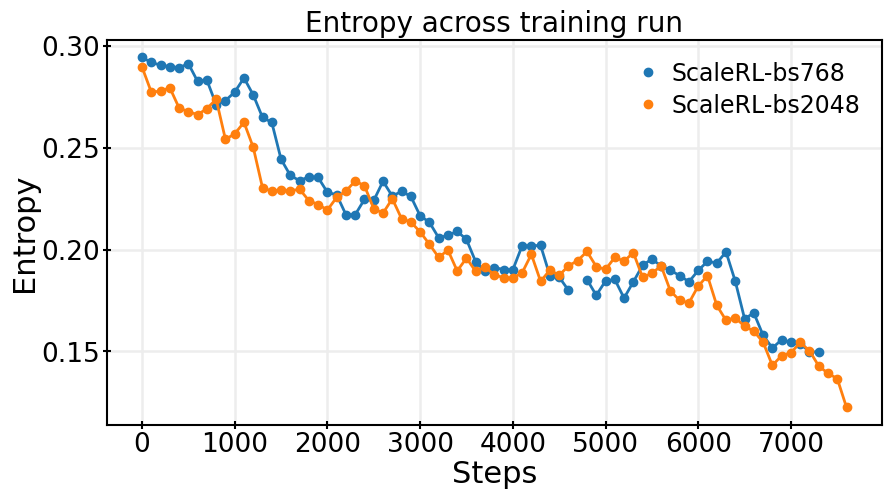
\includegraphics[width=0.7\textwidth]{paper_figs/entropy.png} \label{fig:entropy}
    \hfill
    \caption{Comparing entropy of large and smaller batch size runs across training steps.}
    % \vspace*{-2mm}
\end{figure*}

Overall, our findings suggest that while entropy decreases consistently during training, it is not necessarily a reliable predictor of downstream performance. 
This observation reinforces the need to focus on algorithmic and scaling choices (e.g., batch size, off-policy method) in adddition to entropy dynamics when aiming for improved performance, both on training distribution as well as downstream task distribution.


\begin{figure*}[h]
% \vspace*{-2mm}
    \centering
    \subfloat[]{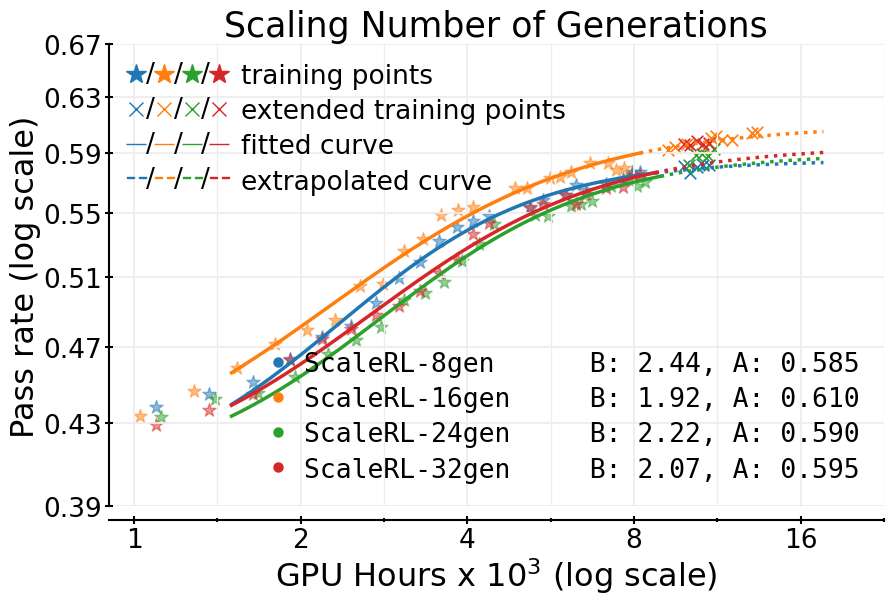
\includegraphics[width=0.51\textwidth]{paper_figs/large_scale_ngens.png}}
    \hfill
    \subfloat[]{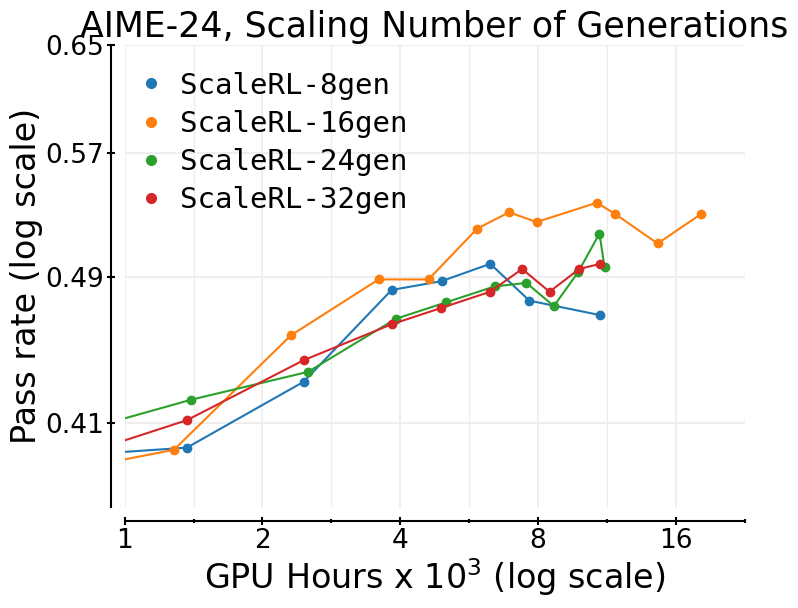
\includegraphics[width=0.47\textwidth]{paper_figs/large_scale_ngens_aime24.png}}
    \hfill
    \caption{Scaling to (a) different number of generations per prompt, (b) Downstream performance of different number of generations per prompt}
    \label{fig:appendix_scaling}
\end{figure*}


\subsection{Scaling on multiple axes}\label{appendix:large_scale}
We provide the remaining scaling to different axes figure here in \Cref{fig:appendix_scaling}, and the corresponding downstream evaluation in \Cref{fig:appendix_scaling_evals}. We also provide the value of $A, B, C_{mid}$ in \Cref{tab:diff_axes}.

\begin{table*}[h]
\centering
\small
\resizebox{0.75\linewidth}{!}{
\begin{tabular}{cccc}
\toprule
Experiment & $C_{mid}$ & $B$ & $A$ \\ \midrule
\scalerl\  & 2542 & 1.92 & 0.610\\
\scalerl-32k  & 11272 & 1.89 & 0.645 \\ 
\scalerl-8gen & 2542 & 2.44 & 0.585\\
\scalerl-24gen  & 3054 & 2.22 & 0.590\\
\scalerl-32gen  & 2936 & 2.07 & 0.595\\
\scalerl-Scout  & 4242 & 1.65 & 0.710\\
\scalerl-bs512  & 2818 & 1.77 & 0.605\\ 
\scalerl-bs2048  & 10909 & 1.70 & 0.645\\ 
\scalerl-math+code, math curve  & 2896 & 2.05 & 0.595 \\
\scalerl-math+code, code curve  & 1675 & 1.09 & 0.615\\
\bottomrule
\end{tabular}
}
\caption{$C_{mid}, B, \text{ and }A$ values for the large scale runs in \Cref{sec:diff_axes}.}
\label{tab:diff_axes} 
\end{table*}

\subsection{Downstream performance} \label{appendix:downstream_perf}

\begin{figure}[h]
    \centering
    \subfloat[]{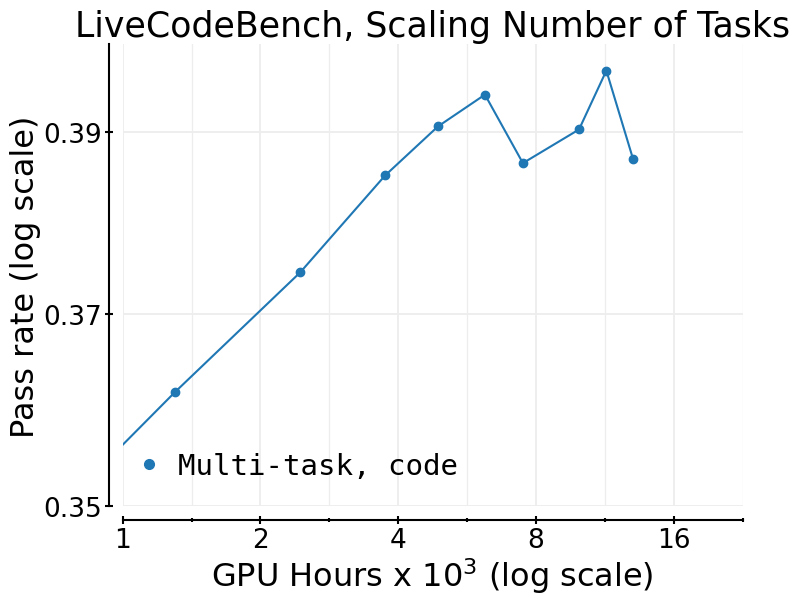
\includegraphics[width=0.45\textwidth]{paper_figs/large_scale_tasks_code_livecodebench.png}}
    \hfill
    \subfloat[]{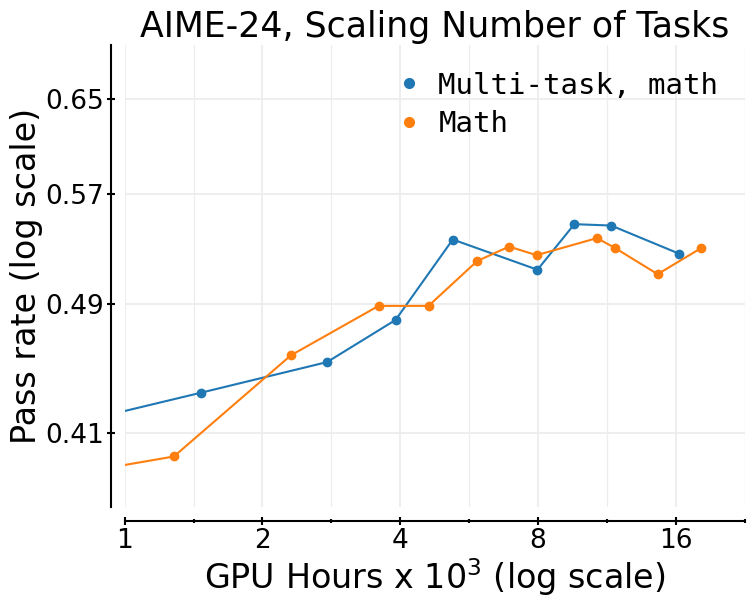
\includegraphics[width=0.45\textwidth]{paper_figs/large_scale_tasks_math_aime24.png}}
    \hfill
    \caption{Downstream performance of (a) different number of generations per prompt, on AIME, (b) LiveCodeBench (Jan-June 2025) performance on math+code run, (c) AIME-24 performance on math+code run}
    \label{fig:appendix_scaling_evals}
\end{figure}


In \Cref{fig_100k_main}, \ref{fig:large_scale_gen_len}, \ref{fig:large_scale_bsz_aime24}, and \ref{fig:appendix_scaling_evals}, we report a representative set of downstream evaluation curves. 
These include \scalerl\ runs with batch sizes $\{512, 768, 2048\}$, long-context training run with $32\text{k}$ generation length, the large-model (Scout) training run, a multi-task run (math + code), and different number of generations per prompt (with fixed batch size) run. 
For each setting we plot performance against compute.
Moreover, we see downstream performance better for experiments like larger batch sizes, longer generation length, and large model size - mirroring similar order for validation set curves.

\subsection{Truncations and training instabilities} \label{appendix:truncations}
Across our experiments we found that training instabilities were often linked to truncations. 
As generation length grew, many RL runs exhibited fluctuating truncation rates that sometimes increased over training. 
At batch size $768$, we observed that truncations in the range of $10$–$15\%$ typically destabilized training, with performance degrading and not recovering without intervention. 
Examples include the extended GRPO run in \Cref{fig:prevelant_methods}, where instability correlated with rising truncation rates, and the updated baseline used in \Cref{sec:fwd_ablations}.

By contrast, \scalerl\ runs were more stable. 
On the $8$B model, truncations remained below $5\%$ for over $90\%$ of training. 
At batch size $2048$, truncations were slightly higher, occasionally approaching $\sim 7\%$. 
This increase was largely attributable to longer average generation lengths observed during training, which naturally raise the chance of exceeding the budget. 
Nevertheless, because the effective batch size (after excluding truncated samples) remained large, training stability was preserved. 
Intuitively, larger generation length budget should help reduce truncations. Training with $34$k generation length (batch $768$) remained stable - truncations briefly spiked to $\sim 4\%$ but quickly fell below $2\%$. 

Larger models were even more robust. 
On the Scout run, truncations remained consistently below $2\%$, and for $>90\%$ of training steps were under $1\%$. 
This likely reflects both the inherent ability of larger models to regulate generation length and their stronger instruction-following ability, which made interruption signals more effective. 

Overall, we suggest practitioners monitor truncation rates closely. 
Our findings indicate that high truncation rates are a reliable warning signal of instability, while larger models, higher generation budgets, and careful design choices (as in \scalerl) substantially mitigate this risk.






\subsection{Comparing Prevalent Methods}\label{appendix:prevelant_methods}
In \Cref{fig:prevelant_methods} we compared some popular training recipes with \scalerl. We briefly describe these existing recipes here.

\paragraph{DeepSeek (GRPO)}
This recipe mostly follows the DeepSeek~\cite{guo2025deepseek} work. We use GRPO as the loss function (\Cref{appendix:background}) with $\epsilon_{min}=\epsilon_{max}=0.2$, sample average loss aggregation, and PPO-offpolicy-8 algorithm. We saw the training became unstable post 6k GPU Hours due to truncations (\Cref{appendix:truncations}).

\paragraph{Qwen2.5 (DAPO)}
This recipe follows DAPO~\cite{yu2025dapo}. It includes the DAPO loss function (Appendix~\ref{appendix:background}) with $\epsilon_{min} = 0.2, \epsilon_{max}=0.26$ (Appendix~\ref{appendix:grpo_eps}). This recipe uses PPO-offpolicy-8, and prompt average loss aggregation. The only change from the original DAPO paper~\citep{yu2025dapo} was regarding dynamically filling in the batch. Specifically DAPO drops 0-variance prompts and samples more prompts until the batch is full. In our codebase, this was not efficent because for PPO-offpolicy algorithm, we had generators pre-decide that each generator will generate rollouts for $\nicefrac{\#\text{prompts}}{\#\text{generators}}$. Therefore, if a specific generator had more 0-variance prompts, it sampled further prompts to complete its share of $\nicefrac{\#\text{prompts}}{\#\text{generators}}$. This could lead to other generators being stalled and an overall slowdown. Hence, to get around this issue, we rather kept a larger batch size of $1280$ (80 prompts, 16 generations each), and dropped 0-variance prompts from the batch. We noted that post-dropping, the effective batch was still greater than 768, what we used for \scalerl. Therefore, if at all, we gave some advantage to the DAPO recipe.

\paragraph{Magistral}
This refers to the recipe used in \cite{rastogi2025magistral}. It includes similar recipe as DAPO with the main difference being PipelineRL used as the off-policy algorithm.

\paragraph{MiniMax}
This refers to the recipe used in \cite{minimax_m1}. It uses CISPO loss, FP32 precision fix at the LM head, PPO-offpolicy algorithm, and prompt average. Similar to DAPO, it drops 0-variance prompts as well and hence we give it a larger batch size of $1280$ as well.


\subsection{Loss Type - Stability and Robustness} \label{appendix:loss_types}

As discussed below, GRPO/DAPO-style losses are highly sensitive to the choice of clipping ratio hyperparameter $\epsilon_{\max}$. 
In contrast, CISPO and GSPO show far greater robustness. 
For example, in Appendix~\ref{appendix:dense_impala}, varying $\epsilon_{\max}$ for CISPO between $\{4,5,8\}$ produced no significant differences in performance. 
For GSPO, the $10^{-4}$ clipping scale used in the original paper~\citep{gspo} did not work well in our setting. We therefore ablated across broader scales and found that once the correct order of magnitude was identified (e.g., $4\!\times\!10^{-3}$ and higher), performance was stable and largely insensitive to fine-grained changes (e.g., $\{4\!\times\!10^{-3}, 5\!\times\!10^{-3}$). 

\begin{figure*}[h]
    \centering
    \subfloat[]{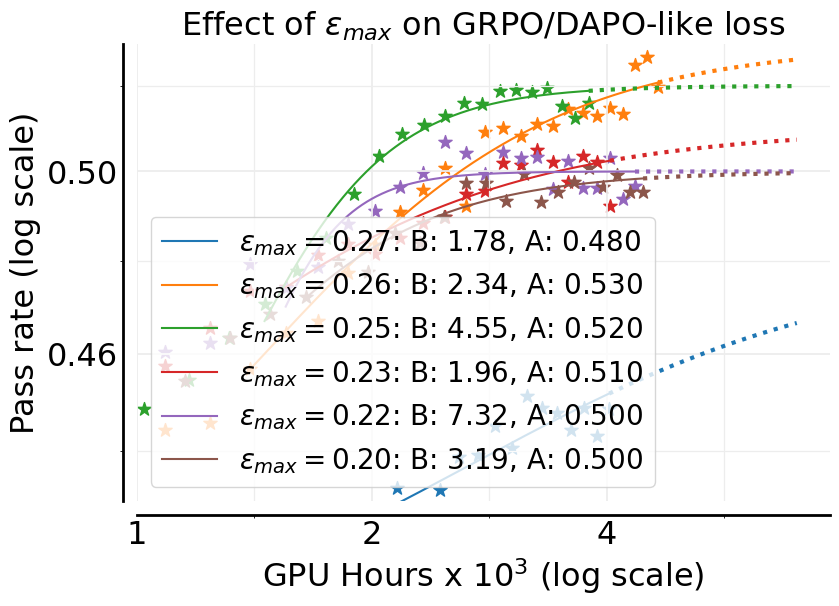
\includegraphics[width=0.49\textwidth]{paper_figs/grpo_eps.png} \label{fig:grpo_eps}}
    \hfill
    \subfloat[]{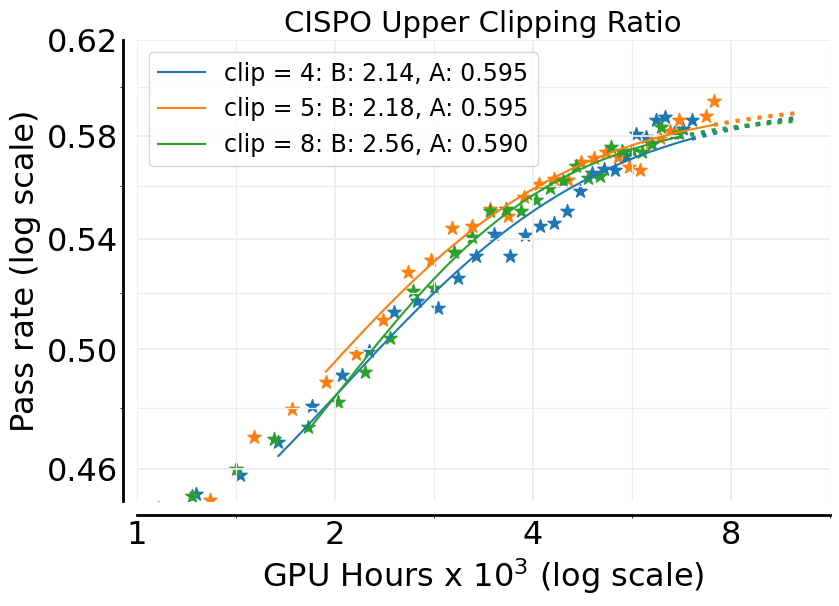
\includegraphics[width=0.49\textwidth]{paper_figs/cispo_eps.png} \label{fig:dense_impala}}
    \caption{(a)Comparing upper clipping ratio of DAPO loss function. Change of $\epsilon_{max}$ fundamentally changes the asymptotic performance value $A$. (b) CISPO clipping ratio ablations}
\end{figure*}



\subsubsection{DAPO clipping ratios} \label{appendix:grpo_eps}
In this section, we analyze the role of the clipping threshold $\epsilon_{\max}$ in DAPO Loss Function~(\cref{eq:dapo_loss}). The hyper-parameter sensitivity of $\epsilon_{max}$ has been observed in prior work, for example, GRPO typically sets $\epsilon_{\max}=0.2$, while DAPO uses $0.28$. However, beyond tuning sensitivity, we find that $\epsilon_{\max}$ directly alters the scaling behavior of the algorithm. 
As $\epsilon_{\max}$ increases, the terminal reward $A$ increases until an optimal range is reached, after which $A$ decreases again. 
This is a striking effect: unlike many hyper-parameters that merely shifts the convergence speed, $\epsilon_{\max}$ governs the asymptotic error itself.



\subsubsection{CISPO Clipping Ratios}\label{appendix:dense_impala}
We ablate the higher clipping ratio for CISPO, keeping the lower clipping ratio fixed at $0$ (\Cref{fig:dense_impala}). 
Across a wide range of values, we find little difference in performance, indicating that CISPO is largely insensitive to this hyperparameter. 
This robustness mirrors our findings for GSPO (\Cref{appendix:gspo_scale}), and stands in contrast to DAPO/GRPO-style objectives, which are highly sensitive to the exact choice of clipping threshold. 
Such stability under hyperparameter variation makes CISPO a strong candidate for default use in large-scale training.


\subsubsection{GSPO ablations} \label{appendix:gspo_scale}
We ablate the clipping-ratio scale used in GSPO, as shown in \Cref{fig:gspo_scale}. The default $10^{-4}$ scale as given in the GSPO paper~\cite{gspo} does not scale the best for our 8B model.
The $10^{-3}$ scale performs as well as, or better than, alternatives (\Cref{fig:gspo_scale})
Given this scale, we further varied the upper clipping ratio in $\{4\!\times\!10^{-3}, 5\!\times\!10^{-3}\}$ and found $\{5\!\times\!10^{-3}\}$ yielded slightly better fit (\Cref{fig:gspo_e_3}).



An important observation is that GSPO is quite robust to the choice of clipping ratio. Once the correct scale is identified, most nearby values or even larger scale perform similarly. 
This robustness contrasts sharply with DAPO-style losses, which are highly sensitive to the exact value of the higher clipping ratio, as noted in \Cref{sec:loss_type}.

\begin{figure*}[h]
    \centering
    \subfloat[]{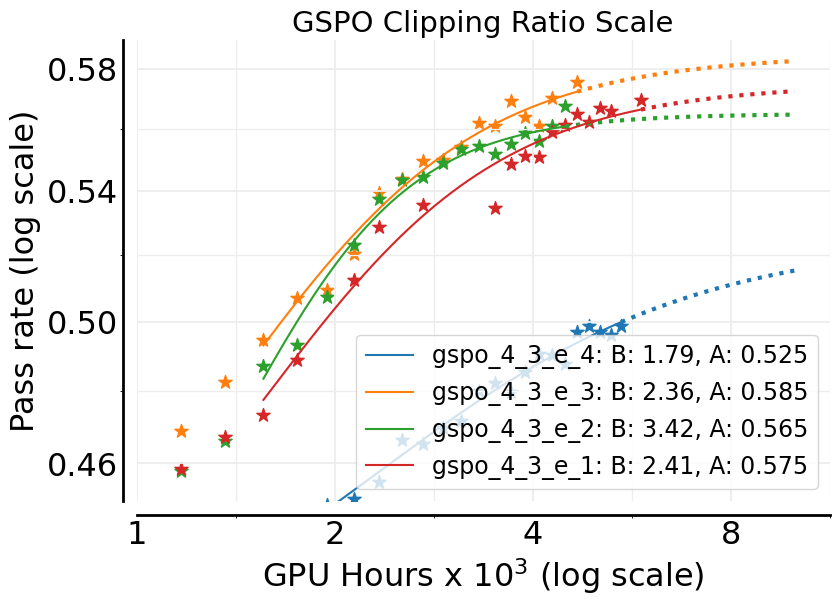
\includegraphics[width=0.49\textwidth]{paper_figs/gspo_eps.png} \label{fig:gspo_scale}}
    \hfill
    \subfloat[]{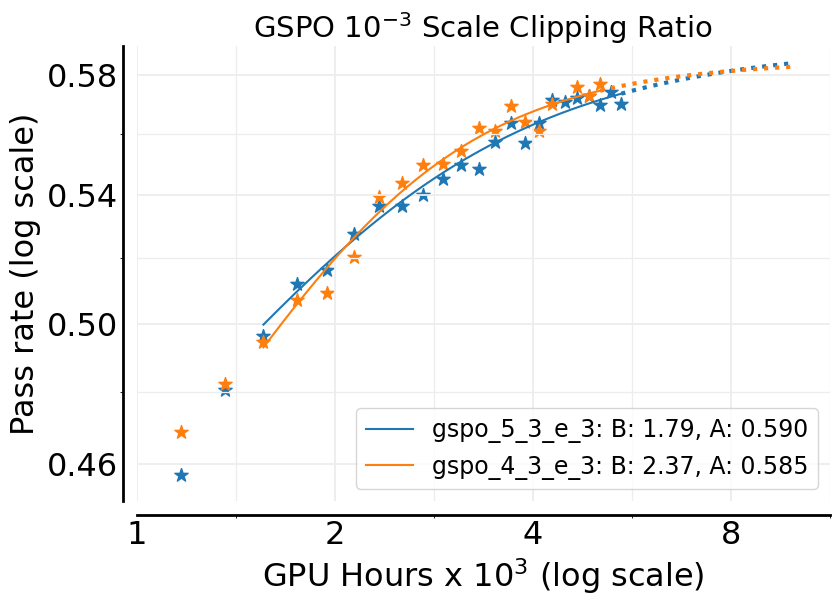
\includegraphics[width=0.49\textwidth]{paper_figs/gspo_e_3.png} \label{fig:gspo_e_3}} 
    \hfill
    \caption{(a) GSPO Scale comparison. gspo\_$x\_y\_e\_z$ in the legend means an upper and lower threshold of $\{x\times 10^{-z}$ and $y\times 10^{-z}\}$ respectively. (b) With $10^{-3}$ scale, we found similar performance for both $4\_3\_e\_3$ and $5\_3\_e\_3$, with latter performing slightly better.}
\end{figure*}


\subsubsection{GSPO vs CISPO} Despite hyperparameter robustness, we encountered stability issues with GSPO. On multiple occasions, GSPO runs diverged mid-training, leading to sudden drops in performance. 
For 8B models, restarting from a stable checkpoint allowed recovery, but this strategy failed on larger models such as Scout, where instability persisted despite repeated resetting to a stable checkpoint.
While we checked to the best of our ability for any implementation bugs, we did not find one.

Overall, while all three loss families can be competitive under tuned settings, CISPO offers the best balance of stability and robustness to hyperparameters, making it our recommended choice.
